\chapter{Algebra \& Trigonometery}\label{apx:algebra}

We'll start simple and build up the complexity to give you an introduction to
some of the basic physical and mathematical concepts that we will need as part
of this course.

\section{Algebra}

While much of this particular tutorial may be review for many of you, it is
important to define the set of rules for our common language.  We will use them
as we rearrange equations on the way to identifying key geophysical
relationships.  If you aren't a math fanatic you are more than likely to find
much of this dreadfully boring (I'm actually falling asleep writing this...but
that could be because it is after midnight).  However, it is important to define
these properties as they will not be true for all operators as we move beyond
simple scalar algebra.  (Remember: a scalar is a single number value
representing a quantity at a single point in space and time).

\subsection{Order of Operations}

Take the following example:
\begin{equation*}
    2 + 3 * 5 = ?
\end{equation*}
Do we work right-to-left or left-to-right?  If we perform the sum first and the
multiplication second, we find
\begin{equation*}
    (2 + 3) * 5 = 5 * 5 = 25 .
\end{equation*}
Note I have used parentheses to specify group the sum so that it is performed
first in this case.  Let us try again, but multiply first and sum second,
\begin{equation*}
    2 + (3 * 5) = 2 + 15 = 17 .
\end{equation*}
These answers are not the same! Hence the order of operations matters.  How do
we choose the order of operations?  The rules are set by convention and the
specific ordering is given in the table below with the highest order operations
to be performed first.  Anything at the same order $+$ and $-$ for example can
be performed interchangably.  If we then follow the order of operations
appropriately, it does not matter if we work right-to-left or left-to-right in
more complex situations.

\begin{table}[hbt]
    \centering
    \caption{Operation hierarchy.\vspace{2pt}}
    \label{tab-symbols}
    \begin{tabular}{ccl}
        \toprule
        order & symbol & operation \\
        \midrule
        1 & $($ $)$, $[$ $]$, $\{$ $\}$ & grouping (inside first) \\
        2 & $a^x$, $\sqrt[x]{a}$, $\dagger$ & powers, roots, conjugation \\
        3 & *, / & multiplication and division \\
        4 & +, - & addition and subtraction \\
        \bottomrule
    \end{tabular}
\end{table}


\subsection{Operators} \label{algebra:ops}

An operation is a task or procedure that results in a new result from one or
more input parameters.  An operator is the symbol/name you instill with a
special functionality.  You are no doubt familiar with the most common
operators, $+$, $-$, $*$, $/$, representing addition, subtraction,
multiplication, and division, respectively.  But there are many others,
logarithms ($\log$) and sine ($\sin$), for example.

At the moment, we will define the properties of certain operations for scalars
and we shall see how they hold up for various systems later.  
\begin{description}
    \item[Identity element:] An operation with the identity element leaves the
    second parameter unchanged by the operation.
    \item[Inverse element:] An operation involving a parameter and its inverse
    element yield the identity element.  Basically it undoes an algebraic
    operation; a principle that is commonly employed to rearrange and/or
    simplify relations.
    \item[Commutative property:] A single operation is commutative if swapping the
    order of the parameters does not change the result.
    \item[Associative property:] When the same operator is used in succession,
    the process is associative if the result is unchanged by the order of
    operations.
    \item[Distributive property] One operator is distributive over another if 
\end{description}

\ntextbox{Real Numbers}{
    \noindent At the moment we will just concern ourselves with the set of
    real numbers, denoted $\mathbb{R}$.  Real numbers are defined as a set
    of all numbers along a continuous number line, both positive and
    negative numbers and including decimal values.  It may seem strange that
    I am defining something so seemingly simple, but as you will see later
    in the course some numbers are not part of the real set.

    \begin{center}
        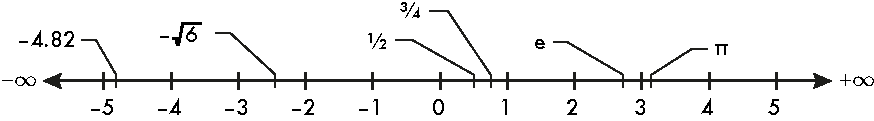
\includegraphics[]{math_primer/figures/real_number_line.pdf}

        \textbf{Figure~\thefigure:} The real number line includes the set of all integers (positive, negative, and zero), fractions, irrationals (e.g.  $\sqrt{2}$), and transcendental numbers (e.g., $\pi$ and $e$).
        \label{fig:realnum}
    \end{center}
}{mathtool}

It would be laborious and unnecessary to prove all of these properties for each
of the the various algebraic operators.  For our purposes, it is sufficient
enough to know that they work...we will leave the proving to the
mathematicians.  So without further ado, rules for addition and multiplication:
\begin{align}
    a + 0 &= a          && \quad \text{identity} \\
    a + b &= b + a      && \quad \text{commutative} \\
    a + (b + c) &= (a + b) + c && \quad \text{associative} \\
    a \cdot 1 &= a      && \quad \text{identity} \\
    ab &= ba            && \quad \text{commutative} \\
    (ab)c &= a(bc)      && \quad \text{associative} \\
    a(b + c) &= ab + ac && \quad \text{distributive}
\end{align}
It is also worthwhile to define multiple self-multiplicative operations, $aa =
a^2$ for instance.  We call these powers---or exponentials for more generally
including non-integer values---which have the properties:
\begin{align}
    a^0 &= 1            && \quad \text{by definition} \\
    a^1 &= a            && \quad \text{identity} \\
    (ab)^c &= a^c b^c   && \quad \text{distributive} \\
    a^b a^c &= a^{(b + c)} && \quad \text{distributive} \\
    (a^b)^c &= a^{(bc)} .
\end{align}
Note the last relation above must be defined, but all others can be derived from
the first set of rules of multiplication.  Many algebraic functions have an
inverse
\begin{align}
    a + b &= c, & b &= c - a; \\
    ab &= c, & b &= c/a; \\
    b^a &= c, & b &= c^{1/a}; \\
    a^b &= c, & b &= \log_a (c) .
\end{align}
Note that are two inverse functions for exponentials, one that allows us to find
the base (former) and one to find the exponent (latter).  There are a few
additional useful properties of logarithms worth mentioning:
\begin{align*}
    \log_a (bc) &= \log_a b + \log_a c , \\
    \log_a (b/c) &= \log_a b - \log_a c , \\
    \log_a (b^c) &= c \log_a b .
\end{align*}

We must also be careful as some operations do not commute, associate, or
distribute over others.  For example: division not distributive over addition,
\begin{equation}
    a/(b + c) \neq a/b + a/c;
\end{equation}
subtraction not commutative,
\begin{equation}
    a - b \neq b - a ;
\end{equation}
and powers not distribute over addition,
\begin{equation}
    (a + b)^c \neq a^c + b^c .
\end{equation}


\section{Trigonometric Functions}\label{apx:trig}

\subsection{Right triangles}

Trigonometric functions are used to relate ratios of the sides to angles.  There
are three primary functions,  
\begin{align*}
    \cos \theta & = \frac{x}{r} , \\
    \sin \theta & = \frac{y}{r} , \\
    \tan \theta = \frac{\sin \theta}{\cos \theta} & = \frac{y}{x}, \\
\end{align*}
where $r$ is the length of the vector, $r = (x^2 + y^2)^{1/2}$ (better known as
they Pythagorean theorem).  The names of these function are the cosine ($\cos$),
sine ($\sin$) and tangent ($\tan$).  The geometrical relationships of the
symbols are defined in Fig.~\ref{fig:triangle}.
\begin{figure}[hbt]
    \centering
    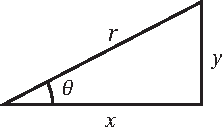
\includegraphics[]{math_primer/figures/trig.pdf}
    \caption{A right triangle.}
    \label{fig:triangle}
\end{figure}
The reciprocal of these relationships also have named functions (secant, $\sec$,
cosecant, $\csc$, and cotangent $\cot$), but are less often used,
\begin{align*}
    \sec \theta = \frac{1}{\cos \theta} & = \frac{r}{x} , \\
    \csc \theta = \frac{1}{\sin \theta} & = \frac{r}{y} , \\
    \cot \theta = \frac{1}{\tan \theta} & = \frac{x}{y} . \\
\end{align*}

We can define the inverse operation of these functions (e.g.\ $\cos^{-1} (\cos
\theta) = \theta$) as
\begin{align*}
    \theta & = \cos^{-1} \frac{x}{r} \\
    \theta & = \sin^{-1} \frac{y}{r} \\
    \theta & = \tan^{-1} \frac{y}{x}. \\
\end{align*}

\subsection{Law of Sines and Cosines}

A couple additional relationships that are useful from time to time are the law
of sines and law of cosines which define the relationships between the length of
the sides and the angles.
\begin{figure}[hbt]
    \centering
    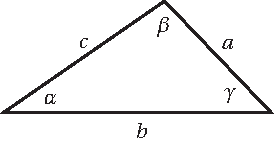
\includegraphics[]{math_primer/figures/trig2.pdf}
    \caption{Any triangle.}
    \label{fig:triangle}
\end{figure}

Law of Sines
\begin{equation*}
    \frac{\sin \alpha}{a} = \frac{\sin \beta}{b} = \frac{\sin \gamma}{c} .
\end{equation*}

Law of Cosines
\begin{equation}
    c^2 = a^2 + b^2 - 2ab \cos \gamma .
\end{equation}

\subsection{Trigonometry and the Unit Circle}

The trigonometric functions can be related to the equation of a circle by
\begin{equation}
    r^2 = \cos^{2} \theta + \sin^{2} \theta,
\end{equation}
where $\cos^{2} \theta = (\cos \theta)^2$ and the angle, $\theta$, measured
counterclockwise from the positive $x$-axis (Fig.~\ref{fig:unitcircle}).  A word
of caution should be given here about notation with respect to powers applied to
trigonometric functions because $\cos^{-1} z \neq (\cos z)^{-1}$ as you will see
below.
\begin{figure}[hbt]
    \centering
    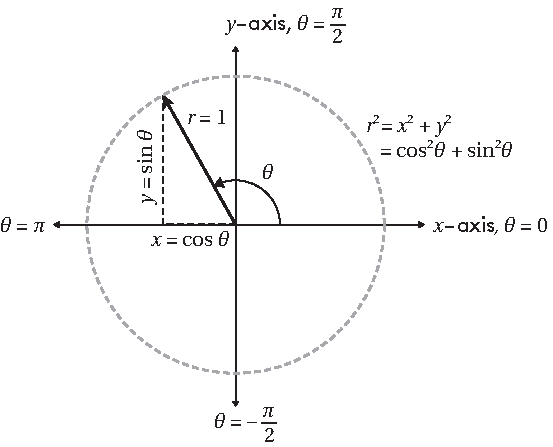
\includegraphics[]{math_primer/figures/unit_circle.pdf}
    \caption{The unit circle and its relationship to trigonometric functions.}
    \label{fig:unitcircle}
\end{figure}

Note: in geophysics, we typically define our angles in radians.  So unless
otherwise specified, assume radians.  There are $2\pi$ radians in a full circle.
Hence 0 is the same direction as $2\pi$, just as 0\deg\ is the same direction as
360\deg.  To convert from one to the other,
\begin{align*}
    \theta(\deg) &= \frac{180}{\pi} \theta(\mathrm{rad}), \\
    \theta(\mathrm{rad}) &= \frac{\pi}{180} \theta(\deg).
\end{align*}

\subsection{Trigonometric Identities}

There are a number of useful trigonometric identites than can be used
to simplify equations.  A selected set from \citet{Zwillinger1996} are included
below.

Pythagorean theorem
\begin{equation*}
    \sin^2 \theta + \cos^2 \theta = 1
\end{equation*}

Angle sum and difference relationships
\begin{align*}
    \sin(\alpha \pm \beta) &= \sin \alpha \cos \beta \pm \cos \alpha \sin \beta \\
    \cos(\alpha \pm \beta) &= \cos \alpha \cos \beta \mp \sin \alpha \sin \beta \\
    \tan(\alpha \pm \beta) &= \frac{\tan \alpha \pm \tan \beta}
        {1 \mp \tan \alpha \tan \beta} \\
    \sin \alpha \sin \beta &= \frac{1}{2} \cos (\alpha - \beta) 
        - \frac{1}{2} \cos (\alpha + \beta) \\
    \cos \alpha \cos \beta &= \frac{1}{2} \cos (\alpha - \beta) 
        + \frac{1}{2} \cos (\alpha + \beta) \\
    \sin \alpha \cos \beta &= \frac{1}{2} \sin (\alpha - \beta) 
        + \frac{1}{2} \sin (\alpha + \beta)
\end{align*}

Double and half angles
\begin{align*}
    \sin 2\theta &= 2\sin \theta \cos \theta 
        = \frac{2\tan \theta}{1 + 2 \tan^2 \theta} \\
    \cos 2\theta &= \cos^2 \theta - \sin^2 \theta 
        = 2\cos^2 \theta - 1 
        = 1 - 2 \sin^2 \theta
        = \frac{1 - \tan^2 \theta}{1 + \tan^2 \theta} \\
    \tan 2\theta &= \frac{2 \tan \theta}{1 - tan^2 \theta} \\
    \sin \frac{\theta}{2} &= \pm \left(\frac{1 - \cos \alpha}{2} \right)^{1/2} \\
    \cos \frac{\theta}{2} &= \pm \left(\frac{1 + \cos \alpha}{2} \right)^{1/2} \\
    \tan \frac{\theta}{2} &= \frac{1 + cos \theta}{\sin \theta}
        = \frac{\sin \theta}{1 - \cos \theta}
        = \pm \left( \frac{1 + \cos \theta}{1 - \cos \theta} \right)^{1/2}
\end{align*}
For half-angles the sign, $\pm$, depends upon quadrant.

Forward--inverse combinations
\begin{align*}
    \sin (\cos^{-1} x) &= (1 - x^2)^{1/2} \\
    \sin (\tan^{-1} x) &= x (1 + x^2)^{-1/2} \\
    \cos (\sin^{-1} x) &= (1 - x^2)^{1/2} \\
    \cos (\tan^{-1} x) &= (1 + x^2)^{-1/2} \\
    \tan (\sin^{-1} x) &= x (1 - x^2)^{-1/2} \\
    \tan (\cos^{-1} x) &= x^{-1} (1 - x^2)^{1/2} \\
\end{align*}

\bibliographystyle{elsarticle-harv}
\bibliography{ref}
